%File: anonymous-submission-latex-2026.tex
\documentclass[letterpaper]{article} % DO NOT CHANGE THIS
\usepackage[submission]{aaai2026}  % DO NOT CHANGE THIS
\usepackage{times}  % DO NOT CHANGE THIS
\usepackage{helvet}  % DO NOT CHANGE THIS
\usepackage{courier}  % DO NOT CHANGE THIS
\usepackage[hyphens]{url}  % DO NOT CHANGE THIS
\usepackage{graphicx} % DO NOT CHANGE THIS
\urlstyle{rm} % DO NOT CHANGE THIS
\def\UrlFont{\rm}  % DO NOT CHANGE THIS
\usepackage{natbib}  % DO NOT CHANGE THIS AND DO NOT ADD ANY OPTIONS TO IT
\usepackage{caption} % DO NOT CHANGE THIS AND DO NOT ADD ANY OPTIONS TO IT
\frenchspacing  % DO NOT CHANGE THIS
\setlength{\pdfpagewidth}{8.5in} % DO NOT CHANGE THIS
\setlength{\pdfpageheight}{11in} % DO NOT CHANGE THIS
%
% These are recommended to typeset algorithms but not required. See the subsubsection on algorithms. Remove them if you don't have algorithms in your paper.
\usepackage{algorithm}
\usepackage{algorithmic}

% Mathematical packages
\usepackage{amsmath}
\usepackage{amssymb}
\usepackage{mathtools}
\usepackage{amsthm}
\usepackage{enumitem}
\usepackage{tikz}
\usepackage{multirow}

% Define theorem-like environments
\newtheorem{definition}{Definition}[section]

%
% These are are recommended to typeset listings but not required. See the subsubsection on listing. Remove this block if you don't have listings in your paper.
\usepackage{newfloat}
\usepackage{listings}
\DeclareCaptionStyle{ruled}{labelfont=normalfont,labelsep=colon,strut=off} % DO NOT CHANGE THIS
\lstset{%
	basicstyle={\footnotesize\ttfamily},% footnotesize acceptable for monospace
	numbers=left,numberstyle=\footnotesize,xleftmargin=2em,% show line numbers, remove this entire line if you don't want the numbers.
	aboveskip=0pt,belowskip=0pt,%
	showstringspaces=false,tabsize=2,breaklines=true}
\floatstyle{ruled}
\newfloat{listing}{tb}{lst}{}
\floatname{listing}{Listing}
%
% Keep the \pdfinfo as shown here. There's no need
% for you to add the /Title and /Author tags.
\pdfinfo{
/TemplateVersion (2026.1)
}

\setcounter{secnumdepth}{0} %May be changed to 1 or 2 if section numbers are desired.

% The file aaai2026.sty is the style file for AAAI Press
% proceedings, working notes, and technical reports.
%

% Title

% Your title must be in mixed case, not sentence case.
% That means all verbs (including short verbs like be, is, using,and go),
% nouns, adverbs, adjectives should be capitalized, including both words in hyphenated terms, while
% articles, conjunctions, and prepositions are lower case unless they
% directly follow a colon or long dash
\title{Markovian Transformers for Informative Language Modeling}
\author{
    Anonymous Submission
}
\affiliations{
    % Anonymous submission - affiliations hidden
}

\begin{document}

\maketitle

\begin{abstract}
  Chain-of-Thought (CoT) reasoning often fails to faithfully reflect a language model's underlying decision process. We address this by introducing a \emph{Markovian} language model framework that can be understood as a reasoning autoencoder: it creates a text-based bottleneck where CoT serves as an intermediate representation, forcing the model to compress essential reasoning into interpretable text before making predictions. We train this system using a policy gradient algorithm inspired by Group Relative Policy Optimization (GRPO), with parallel sampling and actor reward gradients derived from the constraint that our reward model uses the same parameters $\theta$ as the policy model. This approach achieves a 33.2\% absolute accuracy improvement on GSM8K with Llama 3.1 8B. Comprehensive perturbation analysis across 5,888 comparison points and four model pairs demonstrates that Markovian training produces systematically higher sensitivity to CoT perturbations (effect differences +0.0154 to +0.3276), with 52.9\%--87.6\% consistency in showing greater fragility compared to Non-Markovian approaches. Cross-model evaluation confirms that learned CoTs generalize across architectures, indicating they capture transferable reasoning patterns rather than model-specific artifacts.
\
\end{abstract}

% Uncomment the following to link to your code, datasets, an extended version or similar.
% You must keep this block between (not within) the abstract and the main body of the paper.
% \begin{links}
%     \link{Code}{https://aaai.org/example/code}
%     \link{Datasets}{https://aaai.org/example/datasets}
%     \link{Extended version}{https://aaai.org/example/extended-version}
% \end{links}

\section{Introduction}
\label{sec:intro}
The rapid advancement of language models (LMs) has led to impressive performance on complex cognitive tasks~\citep{NEURIPS2020_1457c0d6}. Yet it is often unclear \emph{why} an LM arrives at a particular conclusion~\citep{lamparth2023analyzing,burns2024discovering,gurnee2024language}, causing issues in high-stakes applications~\citep{Grabb2024.04.07.24305462,lamparth2024human,rivera2024escalation}. Traditional interpretability methods analyze hidden activations or attention patterns to extract ``explanations''~\citep{geiger2022inducing,geva2022transformer,meng2022locating,raukur2022toward,wang2022interpretability,lamparth2023analyzing,nanda2023progress}. Modern LMs, however, already generate coherent text: we might hope \emph{prompting} the model to articulate its reasoning (``Chain-of-Thought'' or CoT)~\citep{nye2022show,wei2022chain} would yield a faithful record of its thought process. 

Unfortunately, CoT explanations can be \emph{unfaithful}. For example, \citet{turpin2023language} show that spurious in-context biases often remain hidden in the CoT, and \citet{lanham2023measuring} find that altering CoT text may not affect the final answer. Such observations indicate that standard CoTs are not ``load-bearing.''

In this work, we take a \emph{pragmatic} approach to interpretability, focusing on \emph{informativeness} over full faithfulness. Rather than insisting the CoT mirrors the model's entire internal process, we require that \emph{the CoT alone suffices to produce the final answer}. In other words, if we remove the original prompt and rely only on the CoT, the model should still reach the correct output. This makes the CoT \emph{causally essential} and \emph{fragile}: changing it necessarily alters the prediction.

What distinguishes our approach is the clear distinction between the model \emph{relying on its CoT} versus generating \emph{more informative CoTs}. While traditional approaches train models to generate better-quality CoTs, they don't fundamentally change how the model uses them. Our Markovian framework, by contrast, forces the model to process information through the CoT bottleneck, making the CoT not just informative but \emph{causally load-bearing} for prediction.

For instance, Mistral-7B's CoT on arithmetic tasks changed dramatically after training. \textbf{Before training}, it simply listed all numbers and their (incorrect) sum (e.g., ``Sum = 76 + 90 + 92 + ... = 2314''). \textbf{After training}, it performed correct step-by-step calculations (e.g., ``calculate 6 + 89 = 95; Next, calculate 95 + 38 = 133...''), breaking the task into manageable steps that can be verified independently and enabling accurate answer prediction even when the original question is removed.

\paragraph{Recipient-Specific Compression.}
A key insight is that an \emph{informative} CoT can also serve as a \emph{recipient-specific compression} of the model's hidden knowledge: it distills the essential reasoning into text that another recipient (e.g.\ a different model or a human) can use to predict the same outcome. Our experiments confirm that the learned CoTs generalize across interpreters, suggesting that these textual explanations genuinely encode transferable problem-solving steps rather than model-specific quirks (Section~\ref{subsec:interp}).

\paragraph{Contributions.}
\begin{enumerate}
    \item We introduce a Markovian language model framework that structurally enforces Chain-of-Thought (CoT) generation to be causally essential, ensuring reliance on the CoT for predictions.
    \item We apply this framework to arithmetic problems (Mistral 7B) and the GSM8K dataset~\citep{cobbe2021gsm8k} (Llama 3.1 8B), observing a 33.2\% absolute improvement on GSM8K.
    \item We show through systematic perturbation analysis across four model pairs that Markovian training produces significantly higher sensitivity to CoT perturbations compared to Non-Markovian approaches, with effect differences ranging from +0.0154 to +0.3276 in log-probability sensitivity.
    \item We demonstrate cross-model transfer: CoTs trained on one model remain informative for other models. This underscores the CoT's \emph{recipient-specific} interpretability and suggests it captures a shared reasoning strategy.
\end{enumerate}

Section~\ref{sec:related_work} reviews related work, Section~\ref{sec:MLM} details our Markovian framework, and Section~\ref{sec:method} describes the RL training. Section~\ref{sec:experiments} presents empirical results, and Section~\ref{sec:disc} discusses limitations and future directions.


\begin{figure*}[t!]
  \centering
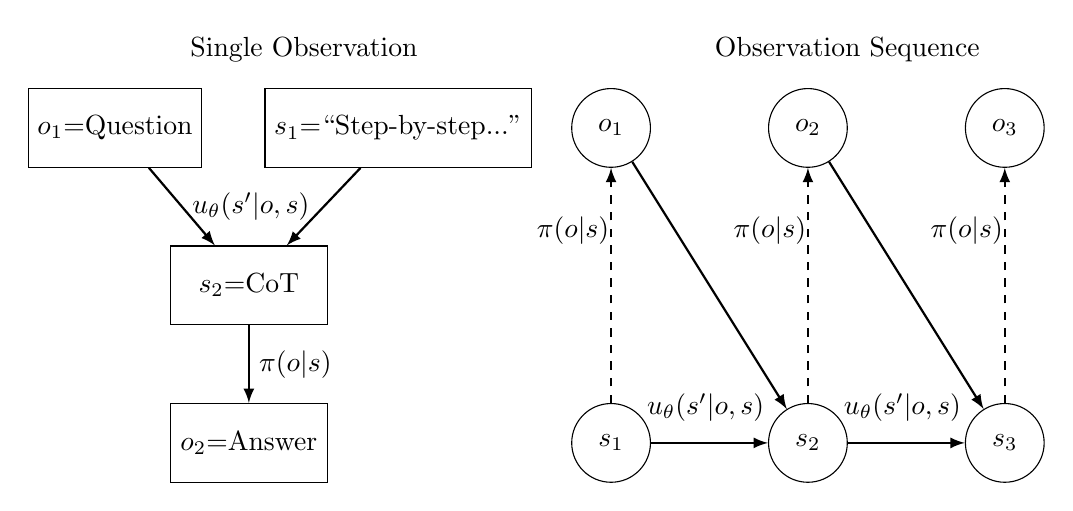
\begin{tikzpicture}[
    node distance=2cm,
    box/.style={rectangle, draw, minimum width=2cm, minimum height=1cm},
    circlebox/.style={circle, draw, minimum size=1cm},
    arrow/.style={->, thick},
    >=latex
]

% Left side: Single timestep
\node[box] (Q) at (-4.3,2) {$o_1$=Question};
\node[box] (S) at (-0.7,2) {$s_1$=``Step-by-step...''};
\node[box] (CoT) at (-2.6,0) {$s_2$=CoT};
\node[box] (A) at (-2.6,-2) {$o_2$=Answer};

\draw[arrow] (Q) -- node[right] {$u_\theta(s'|o,s)$} (CoT);
\draw[arrow] (S) -- (CoT);
\draw[arrow] (CoT) -- node[right] {$\pi(o|s)$} (A);

% Right side: Causal structure
% Observations
\node[circlebox] (o1) at (2,2) {$o_1$};
\node[circlebox] (o2) at (4.5,2) {$o_2$};
\node[circlebox] (o3) at (7,2) {$o_3$};

% States
\node[circlebox] (s1) at (2,-2) {$s_1$};
\node[circlebox] (s2) at (4.5,-2) {$s_2$};
\node[circlebox] (s3) at (7,-2) {$s_3$};

% Connections
\draw[arrow] (o1) to (s2);
\draw[arrow] (s1) to (s2);
\node[above] at (3.2,-1.85) {$u_\theta(s'|o,s)$};

\draw[arrow] (o2) to (s3);
\draw[arrow] (s2) to (s3);
\node[above] at (5.7,-1.85) {$u_\theta(s'|o,s)$};

% π(o|s) connections
\draw[arrow, dashed] (s1) to (o1);
\node[left] at (2.1,0.7) {$\pi(o|s)$};

\draw[arrow, dashed] (s2) to (o2);
\node[left] at (4.6,0.7) {$\pi(o|s)$};

\draw[arrow, dashed] (s3) to (o3);
\node[left] at (7.1,0.7) {$\pi(o|s)$};

% Labels
\node at (-1.9,3) {Single Observation};
\node at (5,3) {Observation Sequence};

\end{tikzpicture}
\caption{Markovian training as a reasoning autoencoder. Left: Single time-step process from Question to CoT to Answer, creating a text-based bottleneck where the CoT must capture all information needed for answer prediction. Right: Causal structure showing the generation of states from observations and previous states using the state update function $u_\theta(s'|o,s)$, and the prediction of observations from states using the policy $\pi_\theta(o|s)$. This architecture forces reasoning through an interpretable text bottleneck, but prevents direct backpropagation, necessitating RL-based gradient estimation. In experiments, both $u_\theta$ and $\pi_\theta$ are implemented using the same transformer (Mistral 7B or Llama 3.1 8B), with only $u_\theta$'s weights updated during training.}
\label{fig:training-method-causal-final}
\end{figure*}

\begin{figure}[t]
  \centering
    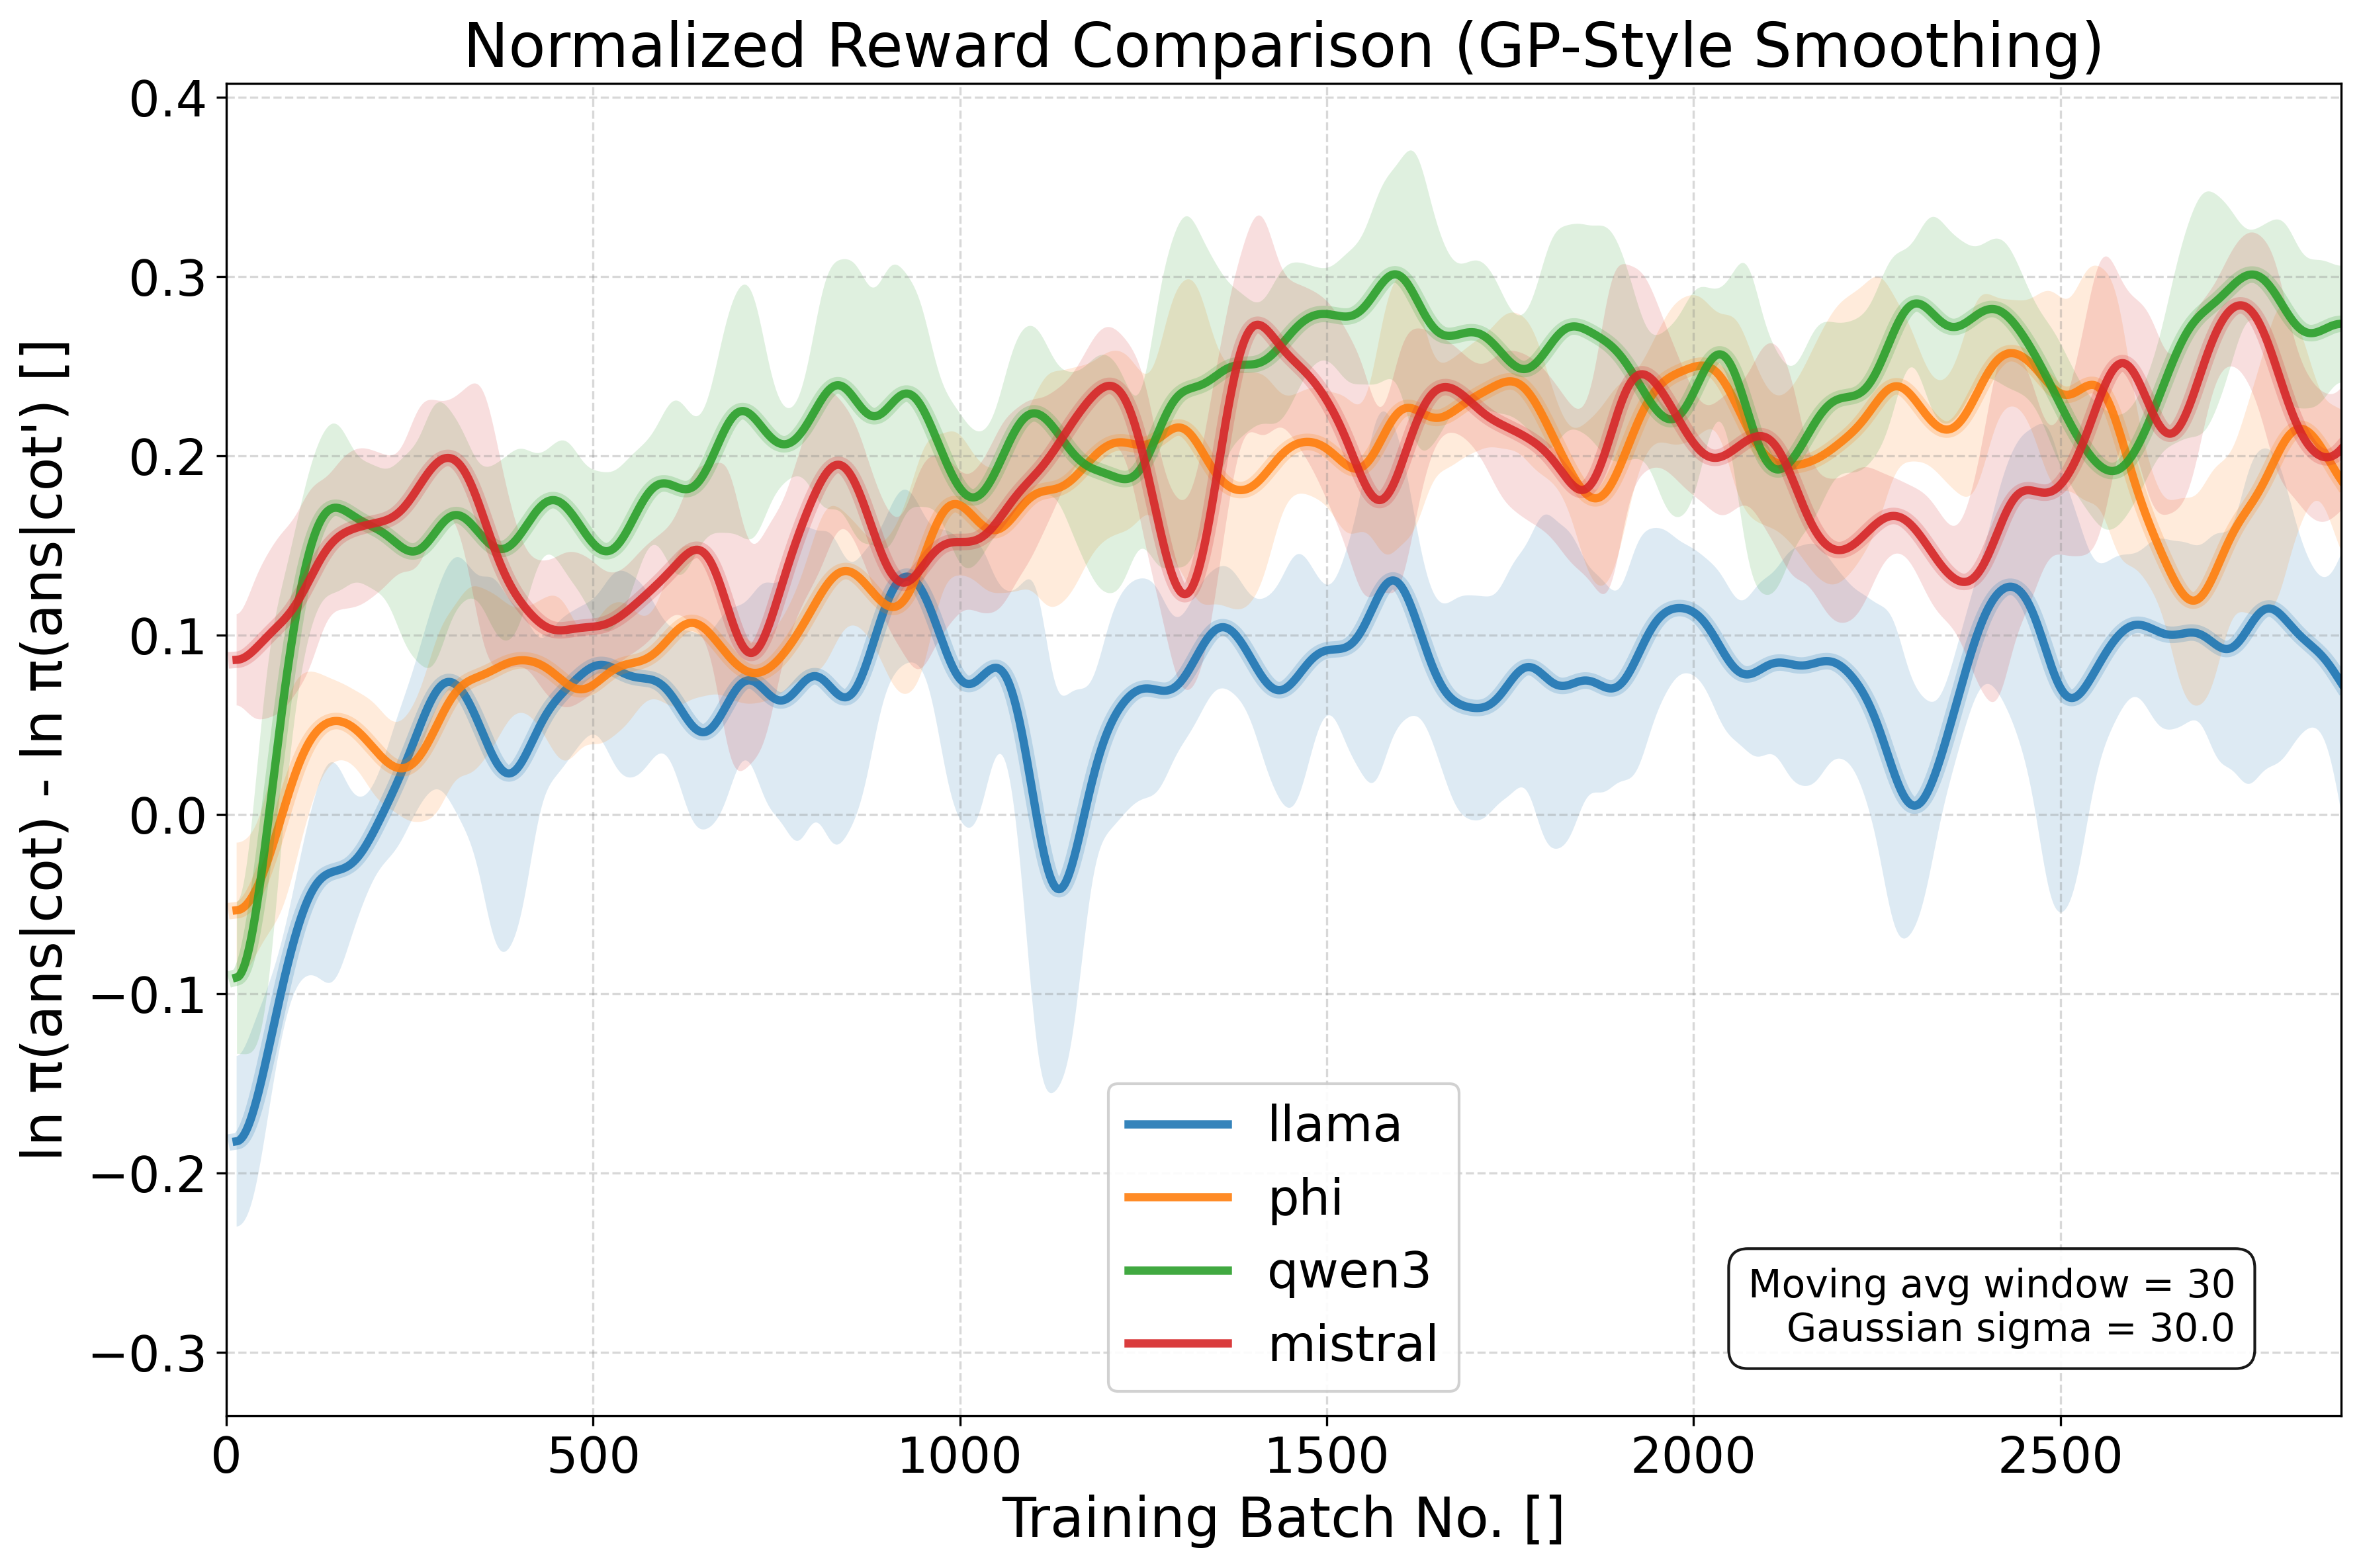
\includegraphics[width=0.43\textwidth]{Figures/combined_normalized_reward_gp_smoothed.png}
    \caption{Normalized reward progression during Wikipedia continuation training across four model architectures. The normalized reward $\ln \pi_\theta(\text{ans} \mid \text{CoT}) - \ln \pi_\theta(\text{ans} \mid \text{CoT}')$ measures how much more informative the trained CoT becomes compared to baseline reasoning from the unmodified model. Each curve represents a different model architecture: Llama 3.1 8B (blue), Phi-3.5 Mini (orange), Qwen3 4B (green), and Mistral 7B (red). The plot uses Gaussian Process-style smoothing with confidence bands to highlight training trends. All models show consistent improvement in CoT informativeness, demonstrating the generalizability of the Markovian training approach across diverse architectures.}
    \label{fig:loss}
\end{figure}

\section{Related Work}
\label{sec:related_work}

Prior work shows that CoT prompting can boost performance on reasoning tasks \citep{wei2022chain, nye2022show}.
Whereas typical CoT prompting methods do not alter a pre-trained model's parameters, some prior approaches do fine-tune the model for CoT generation \citep{eric_star2022, zelikman2024quietstar, deepseekai2025}. Our work differs by removing the original question or passage from the answer-prediction context, which enforces a stronger causal reliance on the CoT.

Regarding faithfulness vs. interpretability, some authors discuss how a CoT may fail to reflect the true reason the LM arrived at its answer \citep{lanham2023measuring, turpin2023language}, since small changes in the CoT do not necessarily change the final prediction. \citet{zhou2023understanding} analyze CoT through an information-theoretic lens, finding that CoT can serve as a communication channel between different parts of a model. We build on these insights by \emph{training} the model to rely on this channel exclusively.

Architecturally, our Markovian LM shares structural similarities with state space models like RNNs \citep{rumelhart1986learning}, S4 \citep{gu2022efficientlymodelinglongsequences}, and Mamba \citep{gu2024mamba}, though with a key difference: MLMs have probabilistic state transitions to model token sampling, which necessitates gradient estimation methods such as policy gradient \citep{policy_gradient} rather than direct backpropagation. This probabilistic structure also resembles Kalman filters \citep{proto_pomdp1965}, Deep Variational Bayes Filters \citep{karl2017deepvariationalbayesfilters}, Deep Kalman Filters \citep{krishnan2015deepkalmanfilters}, and Variational Recurrent Neural Networks (VRNN) \citep{DBLP:journals/corr/ChungKDGCB15}, though we use categorical rather than Gaussian distributions for interpretable text generation. Other fine-tuned reasoning models mentioned above (R1, STaR, and QuietSTaR) have similar structure but allow seeing the full context before generating state/reasoning tokens, whereas our approach enforces a strict information bottleneck through the state.

\citet{lyu2023faithful} also consider restricting the model's ability to see the original input while generating the final answer. Their approach, however, involves rewriting the question in a structured formal language or code that is then executed. Our approach uses natural language for the reasoning state to preserve interpretability across diverse tasks.

\section{Markovian Language Models and Informativeness}
\label{sec:MLM}

Here we provide our formalism for Markovian Language Models (MLMs) and define \emph{informativeness}, which we use as a training objective within our novel structural framework.

\subsection{Markovian Language Models (MLM)}

A traditional LM can attend to the entire context when predicting the next token. This makes it possible for an LM to disregard the CoT or only partially rely on it. We impose a stricter, \emph{Markovian} structure\footnote{This structure can be viewed as a stochastic variant of a Moore machine where both the transition function ($u$) and output function ($\pi$) are probabilistic, and the input and output alphabets are identical ($O$). Alternatively, an MLM can be formalized as an F-coalgebra where F(S) = P(O) $\times$ P(S)$^O$, with P representing probability distributions.}:
\begin{definition}[Markovian LM]
A Markovian Language Model is a tuple $M=(\mathcal{O}, \mathcal{S}, \pi, u, s_1)$, where
\begin{itemize}
\item $\mathcal{O}$ is a set of observations (e.g., questions and answers in a QA task),
\item $\mathcal{S}$ is a set of states (e.g., CoT reasoning text),
\item $\pi: \mathcal{S}\rightarrow \Delta(\mathcal{O})$ is a policy that predicts the next observation from the state alone,
\item $u: \mathcal{O}\times\mathcal{S}\rightarrow \Delta(\mathcal{S})$ is a state update function (produces CoT from question and initial prompt),
\item $s_1\in \mathcal{S}$ is an initial state (starting CoT prompt).
\end{itemize}
\end{definition}

For example, in a math reasoning task, $o_1 \in \mathcal{O}$ might be a question, $s_1 \in \mathcal{S}$ is an initial CoT prompt like ``Let's solve this step-by-step:'', $s_2 \in \mathcal{S}$ is the generated reasoning chain, and $o_2 \in \mathcal{O}$ is the answer. The key idea is that $\pi$ can only see the CoT state $s_2$ when predicting $o_2$, forcing the CoT to contain all needed information. Intuitively, $\pi$ is the \emph{frozen} next-token predictor, and $u$ is the model's \emph{trainable} component that chooses how to produce the CoT from the latest observation and prior state. In our experiments, $\pi$ and $u$ share the same underlying transformer but we freeze the weights for $\pi$ while fine-tuning those used by $u$. 

\subsection{Data-Generating Distribution and Reward}

Let $P$ be the distribution over observations $x_1, x_2, \dots, x_T \in \mathcal{O}$. A trajectory $\tau$ is generated by:
\[
s_{t+1}\sim u(s_t, x_t), \quad x_{t+1}\sim P(x_{t+1}\mid x_{\le t}),
\]
with $s_1$ a fixed initial prompt. We define the \emph{reward} for a trajectory $\tau$ as:
\[
R_\theta(\tau)=\sum_{t=1}^T \left[\ln \pi_\theta(x_t\mid s_t)-\ln \pi_\theta(x_t\mid s'_t)\right],
\]
where $s'_t$ is generated by a \emph{baseline} update function $u'$, e.g., the \emph{untrained} model. In words, $R_\theta(\tau)$ measures how much more likely the correct observation $x_t$ is under the trained state $s_t$ compared to the baseline state $s'_t$.

\subsection{Informativeness Objective}

Conceptually, we aim to ensure that the CoT state serves as a critical bottleneck for information flow, making it causally essential for predictions. Formalizing this within our Markovian framework, we define:
\[
  J(\theta)=\mathbb{E}_{\tau \sim P,u_\theta,u'}\left[R_\theta(\tau)\right],
\]
where $\theta$ parameterizes $u_\theta$. Maximizing $J(\theta)$ ensures that the update function $u_\theta$ produces states $s_t$ that are \emph{informative} about future observations (relative to the baseline $u'$), thereby enforcing the CoT's role as a load-bearing component. We optimize $J(\theta)$ with policy gradient or PPO, sampling observations from $P$ and states from $u_\theta$ and $u'$.

\section{Methods}
\label{sec:method}

\subsection{Implementation as Question-Answer Pairs}
In many tasks like math problem solving, we have $T=2$ observations (question and answer) and implement the abstract MLM with a fixed maximum length for the CoT state. Let $\mathcal{V}$ be a token vocabulary. We set $\mathcal{O} = \mathcal{V}^N$ and $\mathcal{S} = \mathcal{V}^K$ for some $N, K \in \mathbb{N}$, where $K$ is the maximum tokens in the CoT. Note that while we limit the state to a maximum of $K$ tokens for implementation, we do not enforce fixed-length observations. 

Our conceptual arguments rely on $K < N$, as otherwise the model could simply write the predicted observation into the state. We satisfy this in our Wikipedia experiments (Sec~\ref{subsec:wikipedia}), and for other experiments we find empirically that the model does not learn this undesirable behavior due to the difficulty of predicting the answer directly without any CoT.

In this setting, we denote our states as $s_1 = \text{CoT}_{\text{init}}$ and $s_2 = \text{CoT}$, where $\text{CoT}_{\text{init}}$ is a task-specific prompt\footnote{The exact prompt template varies by task type, with each template specifying the task objective, allowed $\text{CoT}$ length, and an invitation to reason strategically. Full templates are provided in Sec~\ref{subsec:stability}.}. With pre-trained LM $\mathcal{L}$, we can implement our update function $u$ and policy $\pi$ using:
\begin{align}
\ln & u \bigl(s_2 = \text{CoT} \,\mid\, q, s_1 = \text{CoT}_{\text{init}}\bigr) \\ &= 
\sum_{i=1}^{K}
    \ln \mathcal{L}\!\Bigl(\text{concat}\bigl(q,\,
    \text{CoT}_{\text{init}},\, \text{CoT}_{<i}\bigr)\Bigr)\bigl[\text{CoT}_i\bigr], \\[1em]
\ln & \pi_\theta (\text{ans} \mid \text{CoT}) \\ &=  \sum_{i=1}^{N} \ln \mathcal{L}(\text{concat}(\text{CoT}, \text{ans}_{<i})) [\text{ans}_i].
\end{align}

Crucially, we do \emph{not} allow the answer generation to attend back to the question $q$ directly; the question is replaced by the $\text{CoT}$. For each question $q$, we generate the baseline state $s'_2$ (which we denote as $\text{CoT}'$ in this setting) by prompting the unmodified pre-trained model with $q$ plus an initial instruction (e.g., 'Think step-by-step...'), and recording its raw output.

Our reward is:
\[
R_\theta = \ln \pi_\theta(\text{ans} \mid \text{CoT}) \;-\; \ln \pi_\theta(\text{ans} \mid \text{CoT}').
\]

\subsection{Policy Gradient with GRPO-Style Baseline}
\label{subsec:grpo}

Markovian training can be understood as training a \emph{reasoning autoencoder}, where the CoT serves as a text-based bottleneck between question and answer. Like traditional autoencoders, this architecture forces information compression, but the intermediate representation is interpretable text rather than latent vectors. This text bottleneck prevents direct backpropagation and necessitates reinforcement learning techniques for gradient estimation.

\subsubsection{Actor Reward Gradients: The Key Innovation}
Our approach differs fundamentally from standard reinforcement learning by using the \emph{same} transformer with weights $\theta$ as both the policy model and the reward model. This creates a crucial mathematical distinction from traditional policy gradient methods.

In classical policy gradient, the reward $R(\tau)$ is independent of the policy parameters, leading to the standard REINFORCE gradient:
$$\nabla_\theta \mathbb{E}_{\tau \sim P_\theta}[R(\tau)] = \mathbb{E}_{\tau \sim P_\theta}[R(\tau) \cdot \nabla_\theta \ln P_\theta(\tau)]$$

However, in our case, the reward is a function of the same parameters: $R_\theta(\tau) = \ln \pi_\theta(\text{ans} \mid \text{CoT})$. Applying the chain rule:
\begin{align}
\nabla_\theta \mathbb{E}_{\tau \sim P_\theta}[R_\theta(\tau)] &= \mathbb{E}_{\tau \sim P_\theta}[R_\theta(\tau) \cdot \nabla_\theta \ln P_\theta(\tau) + \nabla_\theta R_\theta(\tau)]
\end{align}

This yields two terms: the standard policy gradient ($R_\theta(\tau) \cdot \nabla_\theta \ln P_\theta(\tau)$) and the direct reward gradient ($\nabla_\theta R_\theta(\tau)$). We include both terms with equal weight in our implementation.

\subsubsection{GRPO-Style Baseline with Local Subtraction}
We implement a policy gradient algorithm inspired by Group Relative Policy Optimization (GRPO), originally introduced by Shao et al.~\cite{shao2024deepseekmath} in DeepSeek-Math. GRPO eliminates the critic model from PPO by using group-based advantage estimation, where multiple responses to the same query provide relative baselines for each other.

However, we add an additional baseline subtraction step before applying GRPO's batch averaging. We first compute a local baseline using the frozen reference model $u'$, then apply GRPO-style standardization within each batch.

\subsubsection{Parallel Sampling Strategy}
\label{subsubsec:parallel}
We employ \emph{parallel sampling} (inspired by GRPO): each training batch contains $B$ copies of the same question-answer pair $(q, a)$. The trainable model $u_\theta$ generates diverse reasoning chains $\{\text{CoT}_1, \text{CoT}_2, \ldots, \text{CoT}_B\}$ for the identical input through stochastic sampling.

Additionally, we introduce a frozen baseline from the reasoning autoencoder: the unmodified model $u'$ generates a single reference $\text{CoT}'$ that provides a local baseline before applying GRPO-style batch averaging. This frozen baseline represents the "encoder" component of our reasoning autoencoder—capturing the model's initial reasoning ability before training. The frozen baseline $\text{CoT}'$ is \emph{not} part of the original GRPO algorithm—it is our contribution to provide a more stable reference point.

This approach provides several advantages:
\begin{itemize}
    \item \textbf{Reasoning bottleneck}: The $\text{CoT}'$ baseline establishes the initial encoding capacity of the reasoning autoencoder
    \item \textbf{Local baseline}: The frozen $\text{CoT}'$ provides a consistent reference for measuring informativeness improvement
    \item \textbf{Computational efficiency}: Baseline reasoning and answer evaluation are computed once and replicated
    \item \textbf{Stable variance estimation}: All samples share the same ground truth, enabling robust within-batch standardization
\end{itemize}

\subsubsection{Implementation: Two-Term Loss Function}
\label{subsubsec:actor_rewards}
Our implementation combines both gradient terms from the chain rule derivation above. The loss function includes:
\begin{align}
\mathcal{L} &= \mathcal{L}_{\text{PG}} + \mathcal{L}_{\text{AR}} \\
\mathcal{L}_{\text{PG}} &= -\ln u_\theta(\text{CoT} \mid q, \text{CoT}_{\text{init}}) \cdot A^{\text{detach}} \\
\mathcal{L}_{\text{AR}} &= -A
\end{align}
where $A$ is the standardized advantage (after local baseline subtraction and GRPO-style batch averaging) and $A^{\text{detach}}$ blocks gradients to isolate the policy gradient term. 

The first term $\mathcal{L}_{\text{PG}}$ corresponds to the standard REINFORCE gradient $R_\theta(\tau) \cdot \nabla_\theta \ln P_\theta(\tau)$, while the second term $\mathcal{L}_{\text{AR}}$ corresponds to the direct reward gradient $\nabla_\theta R_\theta(\tau)$. This enables simultaneous optimization of CoT generation and answer prediction.

\subsubsection{Within-Batch Advantage Standardization}
Instead of historical exponential moving averages, we standardize advantages within each batch:
\begin{align}
R_i &= \ln \pi_\theta(\text{ans} \mid \text{CoT}_i) - \ln \pi_\theta(\text{ans} \mid \text{CoT}') \\
A_i &= \frac{R_i - \mu_{\text{batch}}}{\sigma_{\text{batch}} + \epsilon}
\end{align}
where $\mu_{\text{batch}} = \frac{1}{B}\sum_{i=1}^B R_i$ and $\sigma_{\text{batch}}^2 = \frac{1}{B}\sum_{i=1}^B (R_i - \mu_{\text{batch}})^2$.

This ensures that advantages have zero mean and unit variance within each batch, providing stable gradients regardless of the absolute reward scale.

\begin{algorithm}
\caption{Policy Gradient with GRPO-Style Baseline}
\label{alg:grpo}
\begin{algorithmic}[1]
\REQUIRE Actor model $u_\theta$ (trainable), Critic model $u'$ (frozen), batch size $B$
\REQUIRE Dataset $\mathcal{D}$, learning rate $\alpha$, temperature $T$, gradient accumulation steps $G$

\FOR{each training iteration}
    \STATE Sample unique example $(q, a) \sim \mathcal{D}$
    \STATE Create batch $\{(q, a), (q, a), \ldots, (q, a)\}$ with $B$ copies
    
    \STATE \textbf{// Generate reasoning chains}
    \FOR{$i = 1$ to $B$}
        \STATE $\text{CoT}_i \sim u_\theta(\cdot | q, \text{CoT}_{\text{init}})$ \COMMENT{Stochastic sampling with temperature $T$}
    \ENDFOR
    \STATE $\text{CoT}' \sim u'(\cdot | q, \text{CoT}_{\text{init}})$ \COMMENT{Deterministic baseline, computed once}
    
    \STATE \textbf{// Calculate informativeness rewards with local baseline}
    \FOR{$i = 1$ to $B$}
        \STATE $R_i = \ln u_\theta(\text{ans} | \text{CoT}_i) - \ln u_\theta(\text{ans} | \text{CoT}')$
    \ENDFOR
    
    \STATE \textbf{// Standardize advantages within batch}
    \STATE $\mu = \frac{1}{B} \sum_{i=1}^B R_i$, \quad $\sigma = \sqrt{\frac{1}{B} \sum_{i=1}^B (R_i - \mu)^2}$
    \STATE $A_i = \frac{R_i - \mu}{\sigma + \epsilon}$ for $i = 1, \ldots, B$ \COMMENT{$\epsilon = 10^{-8}$}
    
    \STATE \textbf{// Calculate loss with actor reward gradients}
    \FOR{$i = 1$ to $B$}
        \STATE $\ell_i^{\text{PG}} = -\ln u_\theta(\text{CoT}_i | q, \text{CoT}_{\text{init}}) \cdot A_i^{\text{detach}}$
        \STATE $\ell_i^{\text{AR}} = -A_i$ \COMMENT{Direct reward optimization}
        \STATE $\ell_i = \ell_i^{\text{PG}} + \ell_i^{\text{AR}}$
    \ENDFOR
    
    \STATE \textbf{// Gradient accumulation and update}
    \STATE $L = \frac{1}{B \cdot G} \sum_{i=1}^B \ell_i$ \COMMENT{Scale by accumulation steps}
    \STATE Accumulate gradients: $\nabla_\theta L$
    \IF{accumulated $G$ steps}
        \STATE Clip gradients: $\|\nabla_\theta\| \leq 1.0$
        \STATE Update: $\theta \leftarrow \theta - \alpha \nabla_\theta$
        \STATE Reset gradient accumulator
    \ENDIF
\ENDFOR
\end{algorithmic}
\end{algorithm}

\subsection{Training Stability and Implementation Details}
\label{subsec:stability}
Fine-tuning a pre-trained language model with a strong linguistic prior requires careful consideration to avoid irrecoverable weight updates that could push the model out of the language modeling loss basin. We implement several techniques to enhance training stability for the GRPO objective:

\begin{enumerate}
    \item \textbf{Low-Rank Adaptation (LoRA) \citep{hu2022lora}:} 
    \begin{itemize}
        \item Freeze all weights except for small-rank LoRA adapters.
        \item Use rank 8 with $\alpha = 16$.
    \end{itemize}

    \item \textbf{Gradient Clipping:} 
    \begin{itemize}
        \item If the $\ell_2$ norm of the gradient exceeds $1.0$, rescale it to norm $1.0$.
    \end{itemize}

    \item \textbf{Gradient Accumulation:} 
    \begin{itemize}
        \item Use gradient accumulation steps of 4 for Wikipedia experiments.
        \item Scale loss by accumulation steps to maintain consistent gradient magnitudes.
    \end{itemize}

    \item \textbf{Within-Batch Advantage Standardization:} 
    \begin{itemize}
        \item GRPO's parallel sampling enables robust within-batch standardization, eliminating the need for historical baselines.
        \item Each batch provides its own reference distribution for advantage calculation.
    \end{itemize}

    \item \textbf{Actor Reward Weight:} 
    \begin{itemize}
        \item Set actor reward weight to 1.0 to equally balance policy gradient and direct reward optimization.
        \item This enables end-to-end learning through the reward model.
    \end{itemize}

    \item \textbf{Initial CoT Prompt Design:} 
    \begin{itemize}
        \item Choose $\text{CoT}_{\text{init}}$ to guide the model toward meaningful reasoning. 
        \item For arithmetic: 
        \begin{quote}
            \small
            ``You will be given an arithmetic problem, which you have [CoT length] tokens to work through step-by-step. Question:''
        \end{quote}
        \item For GSM8K:
        \begin{quote}
            \small
            ``You will be given a reasoning problem, which you have [CoT length] tokens to work through step-by-step. Question:''
        \end{quote}
        \item For Wikipedia continuation:
        \begin{quote}
            \small
            ``Compress your understanding of this text into [CoT length] tokens, then predict the next [target length] tokens.''
        \end{quote}
    \end{itemize}
\end{enumerate}

These measures greatly reduce the risk of catastrophic updates and keep the model's training on track.



\section{Experiments}
\label{sec:experiments}


\subsection{Multi-step Addition}
\label{subsec:solving}
We generate random addition problems, where each problem consists of fifteen terms and each term is a uniform random natural number less than 100. We fine-tune Mistral 7B Instruct V0.2 to produce CoT tokens such that a frozen copy of the pre-trained language model can predict the correct answer given that CoT, for each training technique in Sec~\ref{sec:method}. We plot the mean negative log likelihood over the answer tokens as a function of training batch in Fig.~\ref{fig:loss}. Note that this is both training and testing loss, since we are always generating fresh arithmetic problems. PPO, our preferred training method for arithmetic, can mention the correct answer in up to 90\% of CoTs and achieve an average natural log probability of around -0.7. Additional detailed arithmetic performance analysis is provided in Appendix~\ref{app:additional_figures}. 

Since the Mistral tokenizer allocates a separate token for each digit, a natural log probability of -0.7 corresponds to about 50\% probability ($e^{-0.7} \approx 0.4966$) per token. The seeming contradiction between 90\% verbatim answer likelihood and 50\% per-digit uncertainty stems from the predictor's format uncertainty—it distributes probability across the entire vocabulary when deciding what follows "Answer:", as we only train CoT production $u_\theta(s'|o,s)$, not the predictor $\pi_\theta(o|s)$.

\subsection{GSM8K}
\label{subsec:gsm8k}
To test our method on more complex reasoning tasks, we train Llama-3.1-8B-Instruct on GSM8K using policy gradient with expert iteration (threshold 2.2 standard deviations) and a KL penalty (0.1). We produce up to 150 CoT tokens and estimate the value function with an exponentially decaying average of previous rewards (decay 0.9).

Our experiments show dramatic improvements in exact-match accuracy from 35.94\% baseline to 69.14\% in our best run—a 33.2\% absolute improvement. The other runs (58.23\% and 62.85\%) confirm consistent effectiveness on mathematical reasoning, with CoT informativeness and proportion of CoTs containing verbatim answers both increasing throughout training.

\subsection{Wikipedia}
\label{subsec:wikipedia}

We also explored applying our approach to general language modeling using Wikipedia text. For each article, we condition on the first 200 tokens and task the model with predicting the following 100 tokens, allowing 50 tokens of CoT to aid prediction. Training parameters match those used in GSM8K.

Results showed modest improvements in next-token prediction accuracy from 8.2\% to 10.5\% (see Code and Data Appendix). This should be contextualized against pre-trained Llama's typical 16.9\% accuracy (over 10,000 articles) on the 200\textsuperscript{th} to 300\textsuperscript{th} tokens without context. The lower baseline (8.2\%) likely stems from our setup with CoT followed by `` Answer: '' before prediction. Despite this, key findings about CoT reliability remain evident: as detailed in Sec~\ref{subsec:markovian_sensitivity}, systematic perturbation analysis reveals that Markovian training produces significantly higher sensitivity to CoT perturbations compared to Non-Markovian approaches, indicating genuine structural differences in CoT reliance.
\textbf{See Code and Data Appendix for examples of CoT changes after training.}

\begin{table*}[ht]
  \centering
\small
\begin{tabular}{lcccc}
\hline
\textbf{Perturbation Type} & \textbf{Degree} & \textbf{Mean Effect Difference} & \textbf{Overall Consistency} & \textbf{Total Comparisons} \\
\hline
\textbf{Delete} & 20\% & +0.1193 & 76.1\% & 1,472 \\
& 40\% & +0.2170 & 83.3\% & 1,472 \\
& 60\% & +0.2525 & 84.0\% & 1,472 \\
& 80\% & +0.2612 & 84.8\% & 1,472 \\
& 100\% & +0.3276 & 87.6\% & 1,472 \\
\hline
\textbf{Truncate Front} & 20\% & +0.0317 & 56.4\% & 1,472 \\
& 40\% & +0.0575 & 65.4\% & 1,472 \\
& 60\% & +0.0893 & 70.6\% & 1,472 \\
& 80\% & +0.1457 & 77.7\% & 1,472 \\
& 100\% & +0.3276 & 87.6\% & 1,472 \\
\hline
\textbf{Truncate Back} & 20\% & +0.0154 & 52.9\% & 1,472 \\
& 40\% & +0.0411 & 58.1\% & 1,472 \\
& 60\% & +0.1003 & 64.9\% & 1,472 \\
& 80\% & +0.1681 & 73.4\% & 1,472 \\
& 100\% & +0.3276 & 87.6\% & 1,472 \\
\hline
\textbf{Character Replace} & 20\% & +0.1271 & 76.3\% & 1,472 \\
& 40\% & +0.2245 & 85.9\% & 1,472 \\
& 60\% & +0.2485 & 86.5\% & 1,472 \\
& 80\% & +0.2534 & 86.9\% & 1,472 \\
& 100\% & +0.2548 & 86.9\% & 1,472 \\
\hline
\end{tabular}
\caption{Comprehensive analysis of perturbation sensitivity differences between Markovian and Non-Markovian language model training approaches across four distinct model pairs and four perturbation types. The analysis is based on 5,888 total comparison points (1,472 per perturbation type) collected during training on Wikipedia continuation tasks. \textbf{Mean Effect Difference} represents the average difference in log-probability sensitivity (Markovian effect - Non-Markovian effect), where positive values indicate that Markovian models exhibit greater sensitivity to perturbations. \textbf{Consistency} measures the percentage of training instances where Markovian models showed higher perturbation sensitivity than their Non-Markovian counterparts. Key findings: (1) Delete perturbations show the strongest differences (+0.1193 to +0.3276), (2) Character replacement exhibits robust sensitivity across all severities, (3) Truncation effects are more modest at low severities but converge at high severities, (4) All patterns hold consistently across independent model pairs.}
\label{tab:markovian_comparison}
\end{table*}


\subsection{Markovian vs Non-Markovian Perturbation Sensitivity}\label{subsec:markovian_sensitivity}

To provide systematic evidence for the theoretical advantages of Markovian training, we conduct comprehensive perturbation sensitivity comparisons between Markovian and Non-Markovian model pairs. This analysis directly evaluates whether the structural constraints in Markovian training lead to measurably different robustness properties during training.

\subsubsection{Experimental Design}
We train four independent model pairs on Wikipedia continuation tasks, where each pair consists of architecturally identical transformers differing only in their reward calculation method: Markovian models compute rewards based solely on current token predictions, while Non-Markovian models incorporate full sequence context.

For each training batch, we apply four perturbation types at five severity levels (20\%, 40\%, 60\%, 80\%, 100\%):
\begin{itemize}
    \item \textbf{Delete}: Random token deletion from CoT reasoning
    \item \textbf{Truncate Front}: Removal of tokens from CoT beginning  
    \item \textbf{Truncate Back}: Removal of tokens from CoT end
    \item \textbf{Character Replace}: Random character substitution within tokens
\end{itemize}

The sensitivity measure compares log-probability changes for correct predictions:
\begin{align}
\text{Effect}_{\text{M/NM}} &= \ln P(\text{ans}|\text{CoT}_{\text{original}}) - \ln P(\text{ans}|\text{CoT}_{\text{perturbed}}) \\
\text{Difference} &= \text{Effect}_{\text{Markovian}} - \text{Effect}_{\text{Non-Markovian}}
\end{align}

Positive differences indicate Markovian models exhibit greater sensitivity to perturbations, reflecting stronger reliance on CoT content integrity.

\subsubsection{Results Summary}
Analysis of 5,888 comparison points reveals systematic sensitivity differences between training paradigms. As shown in Table~\ref{tab:markovian_comparison}, delete perturbations produce the strongest effects (+0.1193 to +0.3276 mean difference), with Markovian models showing consistently higher sensitivity that increases with perturbation severity. Character replacement demonstrates robust differences across all severities (+0.1271 to +0.2548), while truncation effects are more modest at lower severities but converge to similar high-severity patterns.

Critically, these patterns hold across all four independent model pairs, indicating systematic rather than coincidental differences. Consistency measures (percentage of cases where Markovian models show higher sensitivity) range from 52.9\% for mild truncations to 87.6\% for severe deletions, providing strong statistical evidence for the theoretical predictions of our framework.

The comprehensive analysis reveals systematic sensitivity differences between training paradigms, with Markovian models consistently exhibiting greater perturbation sensitivity across all tested conditions. These results provide strong empirical support for the theoretical advantages of Markovian training in developing robust reasoning dependencies.

\subsection{Interpretability of CoT Generations}
\label{subsec:interp}

To probe how well the reasoning generalizes, we evaluated the informativeness of Llama's trained CoTs with respect to various other language models on the Wikipedia dataset. Cross-model evaluation shows strong correlation between improvements in both the trained model's and alternative models' evaluations of CoT quality throughout training. The normalized log probabilities increase simultaneously across different architectures, demonstrating that Llama is learning to produce generic CoTs which do not over-fit to the peculiarities of a Llama answer-predictor. Results averaged across 6 independent training runs confirm this pattern holds consistently (detailed results in Appendix~\ref{app:additional_figures}). 

This cross-model transferability addresses a key question: ``interpretable to whom?'' We test across three distinct model families (Phi \citep{abdin2024phi3technicalreporthighly}, Mistral, and GPT2), including GPT2, a significantly smaller model that shouldn't be able to decode sophisticated steganography. The fact that trained CoTs transfer effectively across this diverse set confirms they contain generalizable reasoning patterns rather than model-specific artifacts.

\section{Discussion and Limitations}
\label{sec:disc}

Experiments across arithmetic, GSM8K, and Wikipedia show that it is possible to learn informative and interpretable CoT reasoning via RL on an LM using Markovian training.

However, our interpretability technique is currently only verified in myopic question-answer datasets, as opposed to multi-turn trajectories where trained CoTs might provide a lens into longer-term future behavior. In principle, the Markovian design naturally extends to multi-turn or multi-step settings by treating the CoT as recurrent state; we have not explored such tasks here for scope reasons.

Moreover, we have only evaluated interpretability by measuring \emph{model}-centric proxies (like CoT fragility and cross-model transfer). A more direct human evaluation would have people read the generated CoTs and attempt to predict the final answer, giving an explicit measure of whether these CoTs are genuinely human-interpretable. Such a setup could be incorporated into the training objective, where human correctness in predicting the answer provides an additional signal for optimizing CoT generation.

Markovian training is language modeling with an intermediate memory-producing action, similar to R1 recurrence and ``thinking'' models. This approach blurs the line between RL and unsupervised learning, though its expensive serial token generation requires justification through gains in interpretability or perplexity.

Our findings indicate that Markovian training yields substantial gains in CoT fragility and cross-model transfer, suggesting practical opportunities for improved interpretability. While human studies could further validate interpretability, we rely on cross-model transfer as a proxy and leave comprehensive trials to future work.

\paragraph{Future Work.}
Although we focus on single question–answer pairs, the Markovian framework extends to multi-turn dialogue. After each user message $o_t$, we produce the next CoT $s_{t+1}$ via $u_\theta(s_{t+1}\mid s_t,o_t)$, then generate the system's reply from that CoT alone. This process treats the CoT as a recurrent state, which could scale to conversation rounds.


\bibliography{aaai2026}

\section*{Reproducibility Checklist}

\def\isChecklistMainFile{}
\makeatletter
\@ifundefined{isChecklistMainFile}{
  % We are compiling a standalone document
  \newif\ifreproStandalone
  \reproStandalonetrue
}{
  % We are being \input into the main paper
  \newif\ifreproStandalone
  \reproStandalonefalse
}
\makeatother

\ifreproStandalone
\documentclass[letterpaper]{article}
\usepackage[submission]{aaai2026}
\setlength{\pdfpagewidth}{8.5in}
\setlength{\pdfpageheight}{11in}
\usepackage{times}
\usepackage{helvet}
\usepackage{courier}
\usepackage{xcolor}
\frenchspacing

\begin{document}
\fi
\setlength{\leftmargini}{20pt}
\makeatletter\def\@listi{\leftmargin\leftmargini \topsep .5em \parsep .5em \itemsep .5em}
\def\@listii{\leftmargin\leftmarginii \labelwidth\leftmarginii \advance\labelwidth-\labelsep \topsep .4em \parsep .4em \itemsep .4em}
\def\@listiii{\leftmargin\leftmarginiii \labelwidth\leftmarginiii \advance\labelwidth-\labelsep \topsep .4em \parsep .4em \itemsep .4em}\makeatother

\setcounter{secnumdepth}{0}
\renewcommand\thesubsection{\arabic{subsection}}
\renewcommand\labelenumi{\thesubsection.\arabic{enumi}}

\newcounter{checksubsection}
\newcounter{checkitem}[checksubsection]

\newcommand{\checksubsection}[1]{%
  \refstepcounter{checksubsection}%
  \paragraph{\arabic{checksubsection}. #1}%
  \setcounter{checkitem}{0}%
}

\newcommand{\checkitem}{%
  \refstepcounter{checkitem}%
  \item[\arabic{checksubsection}.\arabic{checkitem}.]%
}
\newcommand{\question}[2]{\normalcolor\checkitem #1 #2 \color{blue}}
\newcommand{\ifyespoints}[1]{\makebox[0pt][l]{\hspace{-15pt}\normalcolor #1}}

\section*{Reproducibility Checklist}

\vspace{1em}
\hrule
\vspace{1em}

\textbf{Instructions for Authors:}

This document outlines key aspects for assessing reproducibility. Please provide your input by editing this \texttt{.tex} file directly.

For each question (that applies), replace the ``Type your response here'' text with your answer.

\vspace{1em}
\noindent
\textbf{Example:} If a question appears as
%
\begin{center}
\noindent
\begin{minipage}{.9\linewidth}
\ttfamily\raggedright
\string\question \{Proofs of all novel claims are included\} \{(yes/partial/no)\} \\
Type your response here
\end{minipage}
\end{center}
you would change it to:
\begin{center}
\noindent
\begin{minipage}{.9\linewidth}
\ttfamily\raggedright
\string\question \{Proofs of all novel claims are included\} \{(yes/partial/no)\} \\
yes
\end{minipage}
\end{center}
%
Please make sure to:
\begin{itemize}\setlength{\itemsep}{.1em}
\item Replace ONLY the ``Type your response here'' text and nothing else.
\item Use one of the options listed for that question (e.g., \textbf{yes}, \textbf{no}, \textbf{partial}, or \textbf{NA}).
\item \textbf{Not} modify any other part of the \texttt{\string\question} command or any other lines in this document.\\
\end{itemize}

You can \texttt{\string\input} this .tex file right before \texttt{\string\end\{document\}} of your main file or compile it as a stand-alone document. Check the instructions on your conference's website to see if you will be asked to provide this checklist with your paper or separately.

\vspace{1em}
\hrule
\vspace{1em}

% The questions start here

\checksubsection{General Paper Structure}
\begin{itemize}

\question{Includes a conceptual outline and/or pseudocode description of AI methods introduced}{(yes/partial/no/NA)}
yes

\question{Clearly delineates statements that are opinions, hypothesis, and speculation from objective facts and results}{(yes/no)}
yes

\question{Provides well-marked pedagogical references for less-familiar readers to gain background necessary to replicate the paper}{(yes/no)}
yes

\end{itemize}
\checksubsection{Theoretical Contributions}
\begin{itemize}

\question{Does this paper make theoretical contributions?}{(yes/no)}
partial

	\ifyespoints{\vspace{1.2em}If yes, please address the following points:}
        \begin{itemize}
	
	\question{All assumptions and restrictions are stated clearly and formally}{(yes/partial/no)}
	yes

	\question{All novel claims are stated formally (e.g., in theorem statements)}{(yes/partial/no)}
	no

	\question{Proofs of all novel claims are included}{(yes/partial/no)}
	no

	\question{Proof sketches or intuitions are given for complex and/or novel results}{(yes/partial/no)}
	yes

	\question{Appropriate citations to theoretical tools used are given}{(yes/partial/no)}
	yes

	\question{All theoretical claims are demonstrated empirically to hold}{(yes/partial/no/NA)}
	yes

	\question{All experimental code used to eliminate or disprove claims is included}{(yes/no/NA)}
	yes
	
	\end{itemize}
\end{itemize}

\checksubsection{Dataset Usage}
\begin{itemize}

\question{Does this paper rely on one or more datasets?}{(yes/no)}
yes

\ifyespoints{If yes, please address the following points:}
\begin{itemize}

	\question{A motivation is given for why the experiments are conducted on the selected datasets}{(yes/partial/no/NA)}
	yes

	\question{All novel datasets introduced in this paper are included in a data appendix}{(yes/partial/no/NA)}
	NA

	\question{All novel datasets introduced in this paper will be made publicly available upon publication of the paper with a license that allows free usage for research purposes}{(yes/partial/no/NA)}
	NA

	\question{All datasets drawn from the existing literature (potentially including authors' own previously published work) are accompanied by appropriate citations}{(yes/no/NA)}
	yes

	\question{All datasets drawn from the existing literature (potentially including authors' own previously published work) are publicly available}{(yes/partial/no/NA)}
	yes

	\question{All datasets that are not publicly available are described in detail, with explanation why publicly available alternatives are not scientifically satisficing}{(yes/partial/no/NA)}
	NA

\end{itemize}
\end{itemize}

\checksubsection{Computational Experiments}
\begin{itemize}

\question{Does this paper include computational experiments?}{(yes/no)}
yes

\ifyespoints{If yes, please address the following points:}
\begin{itemize}

	\question{This paper states the number and range of values tried per (hyper-) parameter during development of the paper, along with the criterion used for selecting the final parameter setting}{(yes/partial/no/NA)}
	partial

	\question{Any code required for pre-processing data is included in the appendix}{(yes/partial/no)}
	yes

	\question{All source code required for conducting and analyzing the experiments is included in a code appendix}{(yes/partial/no)}
	yes

	\question{All source code required for conducting and analyzing the experiments will be made publicly available upon publication of the paper with a license that allows free usage for research purposes}{(yes/partial/no)}
	yes
        
	\question{All source code implementing new methods have comments detailing the implementation, with references to the paper where each step comes from}{(yes/partial/no)}
	partial

	\question{If an algorithm depends on randomness, then the method used for setting seeds is described in a way sufficient to allow replication of results}{(yes/partial/no/NA)}
	partial

	\question{This paper specifies the computing infrastructure used for running experiments (hardware and software), including GPU/CPU models; amount of memory; operating system; names and versions of relevant software libraries and frameworks}{(yes/partial/no)}
	partial

	\question{This paper formally describes evaluation metrics used and explains the motivation for choosing these metrics}{(yes/partial/no)}
	yes

	\question{This paper states the number of algorithm runs used to compute each reported result}{(yes/no)}
	yes

	\question{Analysis of experiments goes beyond single-dimensional summaries of performance (e.g., average; median) to include measures of variation, confidence, or other distributional information}{(yes/no)}
	yes

	\question{The significance of any improvement or decrease in performance is judged using appropriate statistical tests (e.g., Wilcoxon signed-rank)}{(yes/partial/no)}
	no

	\question{This paper lists all final (hyper-)parameters used for each model/algorithm in the paper's experiments}{(yes/partial/no/NA)}
	yes


\end{itemize}
\end{itemize}
\ifreproStandalone
\end{document}
\fi

\end{document}